\section{Considerações iniciais}
A lógica fuzzy foi introduzida por Lofti \citeauthoronline{Zadeh1965} em \citeyear{Zadeh1965}, onde
o autor inicia a discussão definindo os conjuntos fuzzy, as quais constituem classes de objetos com
valores contínuos de pertinência. Cada conjunto é caracterizado por uma função de pertinência, a
qual atribui a cada objeto do conjunto um grau de pertinência que varia entre zero e um. As
operações matemáticas da teoria dos conjuntos, como inclusão, união, intersecção, complemento,
relação, etc., também são estendidas aos conjuntos fuzzy, assim como várias propriedades dessas
notações são definidas.

Uma das motivações para o uso da lógica fuzzy, vem da maneira como nosso cérebro classifica e rotula
o mundo real. Por exemplo, ao rotularmos uma pessoa como alta, estamos atribuindo ela ao grupo de
pessoas altas. Assim como quando nos expressamos sobre o quanto um determinado dia está fazendo
calor ou frio. O conjunto de pessoas altas ou dias frios, não se enquadra na sua totalidade na
lógica clássica, pois essa forma imprecisa de descrever o mundo a nossa volta desempenha um papel
fundamental na forma de pensar humana, assim como também nas áreas de reconhecimento de padrões,
comunicação e abstração \cite{Zadeh1965}.  Neste sentido, esta seção tem como propósito
contextualizar os principais aspectos da lógica fuzzy que a torna tão importante no contexto da
organização flexível de documentos. Ressalta-se, portanto, que definições mais aprofundadas sobre a
lógica fuzzy fogem do escopo desse texto.  Adicionalmente, além dos principais fundamentos
necessários para compreensão da abordagem apresentada neste documento, estão a atividade de
pré-processamento dos dados, cuja finalidade é filtrar e estruturar os dados para serem processados
nas etapas seguintes; os principais algoritmos de agrupamento fuzzy, presentes na literatura, com as
suas definições matemáticas e pseudo códigos; e, por fim, a tarefa de rotular os grupos
encontrados na etapa de agrupamento com os termos que melhor os representem, permitindo assim a
realização de consultas em Sistemas de Recuperação da Informação
(SRI).

\section{Conjuntos e Lógica Fuzzy}

\subsection{Definição de conjuntos fuzzy}

Seja X um espaço de objetos, com um elemento genérico {\it x\/}.  Sendo $X= \big\{x\big\}$.
Um conjunto fuzzy $A$ em $X$ é caracterizado por uma função de pertinência $f_A(x)$, a qual associa
a cada elemento de $X$ um número real presente no intervalo de $[0,1]$, sendo o valor de $f_A(x)$ a
representação do grau de pertinência de $x$ em $A$.

\subsection{Lógica fuzzy}

A lógica fuzzy é uma lógica multi valorada, onde os valores das variáveis pertencem ao intervalo de
$[0,1]$, enquanto na lógica clássica os valores verdades só possuem os estados 0 ou 1 (também
conhecido como valores {\it crisp\/}). Uma da mais importantes aplicações está no tratamento de
precisão e incerteza. O que nos permite modelar soluções mais adequadas para ambientes imprecisos e
incertos.  Antes da lógica fuzzy ser introduzida por \citeonline{Zadeh1965}, em 1930 Lukasiewics
\cite{Chen2000} desenvolveu a lógica n-valorada para $3 < n < \infty$, utilizando apenas os
operadores lógicos de negação $-$ e implicação $\Rightarrow$. Dado então um inteiro positivo, $n >
3$, a lógica n-valorada assume valores verdade pertencente ao intervalo $[0,1]$, definidos pela
seguinte partição igualmente espaçada: $$0 =  \frac{0}{n-1},
\frac{1}{n-1},\frac{2}{n-1},...,\frac{n-2}{n-1},\frac{n-1}{n-1} = 1$$ Para estender a lógica
n-valorada para uma lógica com infinitos valores $2 \leq n \leq \infty$, \citeonline{Zadeh1965}
modificou a lógica de Lukasiewics definindo os seguintes operadores lógicos: 

$$\bar{a} = 1 -a$$ 
$$a \wedge b = min\{a,b\}$$ 
$$a \vee b = max\{a,b\}$$ 
$$a \Rightarrow b = min\{1, 1+b-a\}$$ 
$$a \Leftrightarrow  b = 1 - |a-b|$$

O objetivo da lógica fuzzy é prover mecanismos para tratar imprecisão e incerteza, se baseando na
teoria de conjuntos fuzzy e usando proposições imprecisas, de modo similar a lógica clássica usando
proposições precisas baseadas na teoria dos conjuntos.  Para entender essa noção, observe a seguir
um mesmo exemplo pela ótica do raciocínio clássico e pela ótica das ferramentas usadas para
descrever imprecisão da lógica fuzzy.  

\begin{enumerate}[label=\alph*)] 
\item Todo texto com 100 palavras ou mais da área jurídica, tem como assunto o direito. 
\item O texto A com título ``as manifestações de junho'', tem 100 palavras da área jurídica.  
\item O texto B com título ``política nas universidades'', tem 99 palavras da área jurídica.  
\item O texto A tem como assunto o direito e o texto B não tem como assunto o direito.  
\end{enumerate} 

Essa série de proposições ilustra o raciocínio empregado na lógica clássica e, seguindo as regras de
inferência, conseguimos verificar que as sentenças estão corretas. No entanto, é fácil notar que a
sentença d) não expressa muito bem o nosso entendimento sobre a temática dos textos.  Seria comum
alguém substituir a sentença d), por: O texto B fala um pouco sobre direito.  Sendo assim é possível
adicionar a imprecisão comum no mundo real às sentenças anteriores, conforme reescrito a seguir.

\begin{enumerate}[label=\alph*)] 
\item Todo texto que tem entre 50 e 100 palavras da área jurídica fala um pouco sobre direito.  Enquanto todo texto que contenha 100 ou mais palavras da área jurídica fala bastante sobre direito.  
\item O texto A com título ``as manifestações de junho'', tem 100 palavras da área jurídica.  
\item O texto B com título ``política nas universidades'', tem 99 palavras da área jurídica.  
\item O texto A fala bastante sobre direito, enquanto o texto B fala um pouco sobre direito. 
\end{enumerate} 

Esse tipo de dedução comumente utilizada no nosso dia a dia, não tem como ser tratada pela lógica
clássica. No entanto, podemos lidar com esse tipo de inferência imprecisa, empregando a
lógica fuzzy, a qual permite o uso de alguns termos linguísticos imprecisos como:
\begin{itemize} 
\item Predicados fuzzy: antigo, raro, caro, alto, rápido 
\item Quantificadores fuzzy: muito, pouco, quase, alguns 
\item Graus de verdade fuzzy: totalmente verdadeiro, verdadeiro, parcialmente falso, falso, definitivamente falso 
\end{itemize}

\section{Pré-Processamento} Pré-processamento dos dados é o processo de limpeza e preparação dos
dados para extração de padrões.  Para este trabalho, especificamente, considera-se dado como sendo
um documento textual e a tarefa de extração de padrões a ser considerada é o agrupamento.

Essa etapa é importante porque algumas palavras em um documento podem causar pouco ou nenhum impacto
no significado geral do documento \cite{Haddi2013}.  Soma-se a isso o enorme custo computacional do
processo de mineração de textos, devido à grande quantidade de atributos presente em dados
textuais, visto que quanto maior for a coleção de textos, maior será a quantidade de palavras
distintas. Tal dimensionalidade eleva bastante o custo computacional de qualquer tarefa de extração
de padrões.  Por isso, vários pesquisadores propuseram métodos para tentar simplificar, sintetizar e
eliminar redundâncias desnecessárias nas coleções de textos.  

A fase de pré-processamento voltada para a mineração de textos, as quais visam preparar dados
estruturados para as clássicas operações de mineração de dados, requer técnicas muito específicas
para o preparo dos dados não estruturados \cite{Feldman2007}.

Segundo \citeonline{Feldman2007}, é possível categorizar de maneira clara as técnicas de
pré-processamento de textos em duas categorias, de acordo com as tarefas realizadas pela técnica e
através dos algoritmos e frameworks que a mesma utiliza. Por sua vez, as técnicas categorizadas
pelas suas tarefas, geralmente visam realizar a estruturação do documento através de tarefas e sub
tarefas.  Como por exemplo, realizar a extração de título e sub título de documentos no formato PDF.
No entanto, as demais técnicas de pré-processamento são derivadas de métodos formais, e incluem
esquemas de classificação, modelos probabilísticos e sistemas baseado em regras.

O processo de pré-processamento de dados textuais, inicia com um documento parcialmente estruturado
e avança incrementando a estrutura através do refinamento das características do documento e
adicionando novas \cite{Feldman2007}.  No contexto da mineração de textos, as características dos
documentos são as suas palavras\cite{Haddi2013}. Ao final do processo, as palavras mais relevantes
são utilizadas, e as demais são descartadas.

O processo como um todo envolve várias etapas, as quais pode-se elencar a remoção de espaços,
expansão de abreviações, remoção de $stopwords$, que são palavras que não possuem relevância no
significado geral do texto e geralmente são compostas por proposições, pronomes, artigos,
interjeições dentre outras\cite{Nogueira2013}. Assim como também o processo de $stemming$ ou
lematização, onde se busca encontrar o radical da palavra, visando assim remover palavras que
possuam significados similares. Ainda é possível usar as técnicas de NLP ($Natural Language
Processing$) para eliminar sinônimos. Por fim, é realizada a seleção de termos mais característicos
para toda a coleção \cite{Haddi2013}. 

Diversos métodos foram propostos visando capturar a importância dos termos em coleções textuais.
Sendo o método { \it Term Frequency Inverse Document Frequency\/ }(TF-IDF) um dos mais importantes e
frequentemente utilizado na literatura \cite{Haddi2013}. A definição da TF-IDF está na Equação
(\ref{eq:tfidf}), onde $n$ é o número de documentos da coleção, $DF$ o total de documentos que
possuem este termo e $FF$ ({\it frequency feature}) a frequência do termo no documento.

\begin{equation} 
  \varphi(t,d) = FF * log(\frac{N}{DF}) \label{eq:tfidf} 
\end{equation}

Como resultado final de todo o processo de pré-processamento, obtém-se a matrix $D$. Onde $D$
representa os $n$ documentos da coleção, sendo cada documento $d_{i}$, com $1 \leq i \leq n$, uma
linha da matriz $D$, definido como sendo $ d_{i} =
[\varphi(t_{1},d_{i}),\varphi(t_{2},d_{i}),\varphi(t_{3},d_{i}),...,\varphi(t_{k},d_{i})] $, onde
$t_{j}$ é um termo presente na coleção, com $1 \leq j \leq k$.

\section{Agrupamento Fuzzy} 

O agrupamento é um processo não supervisionado cujo o objetivo é organizar os objetos similares no
mesmo grupo e os objetos com grau de dissimilaridade elevado em grupos distintos
\cite{Nogueira2013}. Este processo é de grande utilidade para diversos campos de estudo da
inteligência computacional, como a mineração de dados, recuperação de informação, segmentação de
imagens e classificação de padrões. Neste trabalho, os objetos a serem agrupados são os documentos
textuais.

O problema de organizar os documentos de maneira a maximizar a similaridade entre os membros de um
mesmo grupo, e minimizar a similaridade entre documentos de grupos distintos, é essencialmente um
problema de otimização.  Sendo assim, pretende-se otimizar a escolha dos grupos, entre
todas as possibilidades de agrupamento, dada uma função objetivo que captura a qualidade dos grupos.
Esta função é responsável por atribuir ao conjunto de possíveis grupos um número real, de maneira
que quanto melhor for os grupos, maior será o seu valor\cite{Feldman2007}.

A medida de similaridade desempenha um papel fundamental no agrupamento, uma vez que ela precisa
expressar o quão distante está um elemento do outro na coleção. Assim sendo, para obtermos bons
resultados durante o processo de agrupamento é de grande importância a escolha adequada da medida
de similaridade, e esta escolha precisa ser feita de acordo com o tipo dos dados.  Na literatura, a
medida de similaridade mais popular é a distância euclidiana (Equação
\ref{eq:euclidiana}), que tem se mostrado bastante adequada em dados com baixa dimensionalidade.

\begin{equation} 
  D(x_{i}, x_{j}) = \sqrt{\sum_k{(x_{ik}-x_{jk})^2}} 
  \label{eq:euclidiana}
\end{equation}

No entanto, em coleções textuais a matriz documentos x termos é naturalmente esparsa, devido a
grande variedade de termos em uma coleção, o que faz com que um determinado documento $d_{i}$ não
contenha diversos termos presentes em um outro documento $d_{j}$. Assim, o vetor de
características de cada documento acaba sendo preenchido com vários zeros, reduzindo a eficácia da
distância euclidiana (Equação \ref{eq:euclidiana}) \cite{Nogueira2013}. 

A medida de similaridade mais comum para coleções textuais é o coeficiente de similaridade de cosseno
\cite{Feldman2007}.  Por sua vez o coeficiente de similaridade de cosseno,
desconsidera os diversos zeros presentes nos vetores de termos dos documentos, levando em conta
apenas o ângulo formado entre eles\cite{Nogueira2013}.  Na Equação (\ref{eq:simcos}) temos a
definição do coeficiente de similaridade de cosseno, onde $d_1$ e $d_2$, são dois documentos
quaisquer da coleção de documentos, e $1 \leq t \leq k$, onde $k$ é a quantidade total de termos da
coleção, e $d_{ik}$ a frequência do termo $t$ no documento $d_i$.

\begin{equation} 
  scos(d_{1}, d_{2}) = cos\theta = \frac{d_{1} \cdot d_{2}}{|d_{1}||d_{2}|} =
  \sum_{t=1}^k{\varphi(d_{1t},d_1) \cdot \varphi(d_{2t},d_2)} \in [0,1] 
  \label{eq:simcos}
\end{equation}

Os grupos resultantes de um  processo de agrupamento, podem possuir algumas características que
estão diretamente relacionadas com o método de agrupamento empregado. Estes podem ser $hard$ ou
$crisp$, caso o método de agrupamento seja baseado na lógica clássica, assim como podem ser $soft$,
caso o método seja baseado na lógica fuzzy. No agrupamento $hard$, cada documento $d_{i}$ só poderá
pertencer a um único grupo $g_{j}$ \cite{Bezdek1984}. Enquanto em grupos $soft$, cada documento
$d_{i}$ pode pertencer a um ou mais grupos $g$, com grau de pertinência variados.  Além destes, os
grupos ainda podem ser $flat$ ou hierárquicos, onde no agrupamento $flat$ todos os grupos estão no
mesmo nível, enquanto no modelo hierárquico os grupos podem estar dispostos em uma hierarquia, de
modo que uma relação de parentesco é definida entre eles.

Para o agrupamento $hard$, considere $G = \{g_{1},g_{2},g_{3},...,g_{c}\}$ os grupos resultantes do
agrupamento, sendo $c$ o total de grupos, e a pertinência de cada documento $d_{i}$ à um grupo
$g_{l}$, $1 \leq l \leq c$, pode ser representada pela função característica $\kappa(d_{i}, g_{j})
\in \{0,1\}$.  Um dos mais populares algoritmos a implementar essa abordagem é o K-Means. Nos
trabalhos de \citeonline{Bezdek1984,Nogueira2013,Feldman2007}, é apontada uma falha inerente dessa
abordagem, pois quando um documento só pode pertencer a um único grupo, fica evidenciado que o mesmo
não compartilha nenhuma similaridade com os documentos dos demais grupos, o que não expressa a
imprecisão intrínseca da sobreposição dos assuntos em documentos de texto.

Com o objetivo de tratar essa falha da abordagem $hard$ e adicionar o tratamento de imprecisão e
incerteza no agrupamento, \citeonline{Bezdek1984} utilizou o modelo de partições fuzzy definido em
\citeonline{Zadeh1965}, para permitir pertinências parciais de um elemento a um grupo, propondo
assim o algoritmo Fuzzy C Means (FCM).  Sendo assim, a função característica passa a ser considerada
como uma função de pertinência de um documento $d_{i}$ em um grupo $g_{l}$, a qual é definida por
$\mu(d_{i}, g_{l}) \in [0,1]$, tal que $\sum_{l=1}^c \mu(d_{i}, g_{j}) = 1$.

Um desafio sempre presente em métodos de agrupamento é a descoberta do número ideal de grupos em uma
coleção. O método de organização flexível proposto em \citeonline{Nogueira2013}, utiliza a  $Fuzzy\
Silhouette$ (FS) para realizar a validação do agrupamento fuzzy, e por conseguinte encontrar o
número de grupos ideal. A função FS é uma adaptação do método de critério de largura média
($Average\ Silhuette\ Width\ Criterion$ - ASWC), desenvolvido para o agrupamento $crisp$. A
definição da silhueta fuzzy está nas Equações (\ref{eq:silhuette}) e (\ref{eq:fs}), onde
$\alpha(d_i, g_l)$ é a distância média entre o documento $d_i$ e todos os documentos presentes no
grupo $g_l$, enquanto $\beta(d_i,g_l) = min\{\alpha(d_i,g_h) | 1 \leq h \leq c; h \neq l\}$, é a
medida de dissimilaridade de $d_i$ ao grupo vizinho mais próximo de $g_l$, tal que $c$ é a
quantidade de grupos.  


\begin{equation} 
  S(d_i) = \frac{\beta(d_i, g_l) - \alpha(d_i,g_l)}{max\{\alpha(d_i,g_l), \beta(d_i,g_l)\}} 
  \label{eq:silhuette}
\end{equation}

\begin{equation} 
  FS = \frac{\sum_{i=1}^n{(\mu_1(d_i) - \mu_2(d_i))}S(d_i)}{\sum_{i=1}^n{(\mu_1(d_i) - \mu_2(d_i))}}
  \label{eq:fs}
\end{equation} 

Na Equação (\ref{eq:fs}), $\mu_1(d_i)$ é a maior pertinência do documento $d_i$ em um grupo,
enquanto $\mu_2(d_i)$ é a segunda maior. Quanto maior então for o valor da função FS, melhor será o
agrupamento. Deste modo, para encontrar o número de grupos ideal, basta executar a função FS
variando o número de grupos, e selecionar o agrupamento que tiver o valor máximo de FS.

Toda investigação realizada neste trabalho tomou como base os métodos de agrupamento que derivam do
algoritmo FCM\cite{Bezdek1984}, descrito a seguir, para se beneficiar da capacidade de tratar
imprecisão e incerteza da lógica fuzzy, e por conseguinte permitir que um mesmo documento seja
categorizado em mais de um tópico (grupo), refletindo a realidade dos documentos textuais. 

Em todos os experimentos a medida de similaridade de cosseno (Equação \ref{eq:simcos}) foi
utilizada, e a quantidade de grupos ideal foi escolhida utilizando o método da silhueta fuzzy (
Equação \ref{eq:fs}).

\subsection{Algoritmo Fuzzy C Means (FCM)} 

\citeonline{Bezdek1984} descreve um método de agrupamento fuzzy
que produz como saída partições fuzzy e protótipos dos grupos. Esse algoritmo desempenha um papel
importante no contexto do agrupamento fuzzy, devido ao seu pioneirismo no campo de estudo, possuindo
diversas extensões, sendo considerado um dos mais amplamente utilizados métodos de
agrupamento fuzzy da literatura\cite{Pal2005}. A maioria dos métodos de agrupamento fuzzy são
derivações do FCM\cite{Krishnapuram1993}.

Para compreensão do algoritmo, considere $V = \{v_1,v_2,v_3,...,v_c\}$ os protótipos dos grupos $G =
\{g_1,g_2,g_3,...g_c\}$ definidos por 

\begin{equation} 
  V = \left\{ v_j | v_j = \frac{\sum_{i=1}^n[\mu(d_i,g_j)]^m d_i}{\sum_{i=1}^n[\mu(d_i,g_j)]^m}, 
  1 < j \leq c \right\}, 
  \label{eq:prototipos} 
\end{equation}
tal que $v_j$ seja o protótipo de $g_j$, $c$ o número de grupos gerados no agrupamento e $n$ o
número de documentos presentes na coleção. 

Seja $U_{c \times n}$ uma partição fuzzy conforme a Equação:

\begin{equation} 
  U_{c \times n} = \{\mu(d_i, g_k) |\mu(d_i, g_k) \in [0,1], 1 < i \leq n, 1 < k \leq c\} 
  \label{eq:part_fuzzy} 
\end{equation} 

Esta partição apresenta todas as pertinências dos documentos aos grupos, cuja função de 
pertinência $\mu(d_i,g_k)$ de cada documento na coleção, é definida por 

\begin{equation} 
  \mu(d_i,g_k) = \frac{1}{\sum_{j=1}^n(\frac{dist(d_i,v_k)}{dist(d_i,v_j)})^{\frac{1}{m-1}}} 
  \label{eq:pertinencia}
\end{equation}
e está sujeita as restrições definidas nas equações (\ref{eq:fcmrestri1}) e (\ref{eq:fcmrestri2}).

Considera-se $m$ o fator de fuzificação, que regula o quão fuzzy serão as partições finais. De modo
que para $m = 1$ a partição resultante é totalmente $crisp$ (Figura \ref{fig:cluster_crisp}) e para
$m \rightarrow \infty$ a interseção entre os grupos tende a aumentar (Figura
\ref{fig:cluster_fuzzy})\cite{Pal2005}. 

Segundo \citeonline{Bezdek1984} nenhuma teoria ou evidência computacional aponta para um valor ótimo
de $m$, contudo o autor aponta que a faixa de valores ideais aparenta ser $[1,30]$. Sendo assim, se
existir um conjunto de dados para teste, uma boa estratégia para a escolha de $m$ é a realização de
testes experimentais. Caso contrário, o intervalo de $[1.5, 3.0]$ aparenta trazer bons resultados
para a maior parte dos dados.

\begin{figure}[!htp] \centering 
   \begin{minipage}{0.45\textwidth} 
     \centering
    \includegraphics[width=0.6\columnwidth]{assets/clusters_crisp.pdf} 
    \caption{Ilustração denotando os
grupos $g_1,g_2,g_3$ organizados sem sobreposição, para $m = 1$.} 
  \label{fig:cluster_crisp}
  \end{minipage}\hfill 
  \begin{minipage}{0.45\textwidth} \centering
    \includegraphics[width=0.6\columnwidth]{assets/clusters_fuzzy.pdf} 
    \caption{Ilustração denotando os
     grupos $g_1,g_2,g_3$ organizados de maneira fuzzy, com sobreposição, quando 
     $m \rightarrow \infty$.}
     \label{fig:cluster_fuzzy} 
   \end{minipage} 
\end{figure}

Usualmente, no contexto do agrupamento de coleções textuais, $dist(d_i,g_k) = scos(d_i,g_k)$.
Adicionalmente, o algoritmo FCM estabelece algumas restrições: deve-se evitar que o FCM produza
grupos vazios (Equação (\ref{eq:fcmrestri1})) e deve-se impor que a soma das pertinências seja
sempre igual a um (Equação (\ref{eq:fcmrestri2})).

\leavevmode\\
\begin{equation} \sum_{k=1}^c
  \mu(d_i,g_k) = 1 \label{eq:fcmrestri1} 
\end{equation}

\begin{equation} 0 < \sum_{i=1}^n
  \mu(d_i,g_k) < n \label{eq:fcmrestri2} 
\end{equation}. 
\leavevmode\\

A restrição imposta pela Equação (\ref{eq:fcmrestri2}), no entanto, produz um problema em elementos
equidistantes aos grupos. Ou seja, quando temos o caso $\mu(d_i, g_1) = \mu(d_i, g_2) = ... =
\mu(d_i, g_c)$. Nessa situação, o grau de pertinência de um elemento a cada grupo será a pertinência
média, ou seja $\mu(d_i, g_1) = \mu(d_i, g_2) = ... = \mu(d_i, g_c) = \frac{1}{c}$. Supondo agora um
segundo documento $d_2$, que seja mais distante do que $d_1$, porém assim como $d_2$, também
equidistante aos grupos, temos que $\mu(d_2, g_j) = \mu(d_1, g_j) = \frac{1}{c}$, para $1 < j \leq
c$. Nesse contexto, a pertinência de $d_2$ e $d_1$, não expressa a distância relativa desses
documentos aos grupos. Esse problema está ilustrado na Figura \ref{fig:fcm_problem}.

\begin{figure}[!htp] \centering
  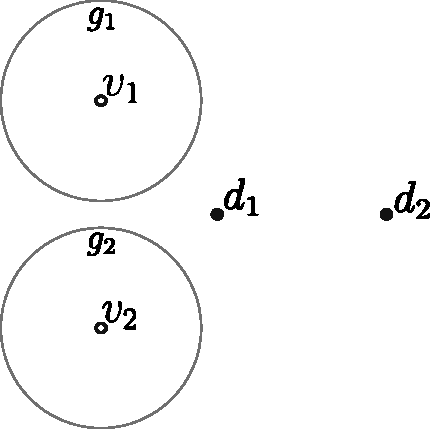
\includegraphics[width=0.4\columnwidth]{assets/fcm_problem.pdf} 
  \caption{Problema dos
    elementos equidistantes do algoritmo FCM. Na imagem $g_1$ e $g_2$ são grupos, com os seus
    respectivos protótipos $v_1$ e $v_2$. Enquanto $d_1$ e $d_2$ são documentos equidistantes aos
    protótipos $v_1$ e $v_2$. Portanto $\mu(d_1,g_1) = \mu(d_1,g_2) = \mu(d_2,g_1) = \mu(d_2,g_2) =
0.5$.} 
  \label{fig:fcm_problem} 
\end{figure}

Segundo \citeonline{Bezdek1984} várias funções de otimização da partição fuzzy produzida no
agrupamento foram propostas, sendo a minimização da função objetivo $J(U_{c \times n},G,V,D)$, 
definida na Equação (\ref{eq:fcm_obj}) a mais popular. Onde considere $U_{c \times n}$ como os graus
de pertinência fuzzy, $V$ os protótipos dos grupos $G$ e $D$ o conjunto de documentos.  

\leavevmode\\
\begin{equation} min\{(J(U_{c \times
n},G,V,D) = \sum_{i=1}^n \sum_{j=1}^c [\mu(d_i, g_j)]^m dist(d_i, v_j)\} 
\label{eq:fcm_obj}
\end{equation} 
\leavevmode\\

O algoritmo mais comumente utilizado para prover soluções aproximadas dessa minimização
(\ref{eq:fcm_obj}), é a através da iteração de Picard\footnotemark \cite{Pal2005} entre as equações
(\ref{eq:prototipos}) e (\ref{eq:part_fuzzy}). 
\footnotetext{Método iterativo para construção de soluções aproximadas, atribuído ao matemático
francês Charles Emile Picard (1856-1941).
\url{http://mathfaculty.fullerton.edu/mathews/n2003/PicardIterationMod.html}} 
O ciclo de aproximações se dá por $V_{t-1} \Rightarrow  U_t \Rightarrow  V_t$, onde, ao final de
cada iteração, é verificado se $\parallel V_{t-1} - V_t\parallel < \varepsilon$.  A literatura
também expressa que os ciclos podem começar pela partição fuzzy, fazendo então $U_{t-1} \Rightarrow
V_t \Rightarrow U_t$, e, ao final do ciclo, checando o erro mínimo com $\parallel U_{t-1} -
U_t\parallel < \varepsilon$, sendo $t$ o contador de iterações.  Contudo, existem benefícios em
termos de processamento e memória ao utilizar a iteração iniciando e finalizando com
$V$\cite{Pal2005}. Por outro lado, \citeonline{Bezdek1984} e \citeonline{Pal2005} afirmam que a
convergência desse modelo iterativo ocorre em ambos os tipos de ciclo. Geralmente, a partição fuzzy
inicial $U_0$ é comumente inicializada com valores aleatórios ou com o resultado de um agrupamento
previamente executado \cite{Pal2005,Krishnapuram1993}. Nas demais iterações a atualização dos
protótipos é realizada a partir da Equação (\ref{eq:prototipos}).  

O pseudo código utilizando a abordagem iterativa descrita a cima, está listado no Algoritmo
\ref{alg:fcm}, no qual a função $\textbf{{\color{blue}inicializa-particao-fuzzy}(D,G)}$, pode ser
uma das duas formas de inicialização descritas anteriormente.

\leavevmode\\
\begin{algorithm}[H] 
  \SetAlgoLined 
  \textbf{{\color{blue}fcm}(D, c, m, $\varepsilon$)}\\
  \Begin{
    G $\gets$ $[g_1,g_2,...,g_c]$\; 
    $U_0$ $\gets$ \textbf{{\color{blue}inicializa-particao-fuzzy}(D,G)}\; 
    $t \gets 0$\; 
    \Do{ $\parallel U_{t-1} - U_t\parallel > \varepsilon$ }{ 
      $V_t$ $\gets$ calcula usando (\ref{eq:prototipos})\; 
      $t \gets t + 1$\; 
      $U_t$ $\gets$ calcula usando (\ref{eq:part_fuzzy})\; 
    }
    $\textbf{retorne} (U_t, V_t)$\; 
  }
  \caption{Pseudo código da implementação iterativa do método FCM}
\label{alg:fcm} 
\end{algorithm} 
\leavevmode\\

Por fim, está ilustrado na Figura \ref{fig:samples_fcm}, os resultados produzidos pelo algoritmo
FCM, em dois conjuntos de coordenadas no $R^2$. Na figura, os pontos foram pintados com a cor
correspondente ao grupo em que o mesmo obteve o maior valor de pertinência.

\leavevmode\\
\begin{figure}[!htp] 
  \centering 
  \includegraphics[width=0.8\columnwidth]{assets/samples_fcm.png}
  \caption{Resultado do agrupamento de dois conjuntos de coordenadas no $R^2$ usando o algoritmo
  FCM\protect\footnotemark.} 
  \label{fig:samples_fcm} 
\end{figure}
\leavevmode\\

\subsection{Algoritmo Possibilistic C Means (PCM)}

A restrição probabilística do FCM, apresentada na Equação (\ref{eq:fcmrestri2}), que obriga a soma
das pertinências de um elemento ser igual a um, nem sempre resulta em pertinências que representam
bem a realidade dos dados, conforme exemplificado na Figura \ref{fig:fcm_problem}.  Esse problema se
agrava ainda mais, em bases com muitos dados ruidosos ($outliers$). Portanto, com o objetivo de
contornar esses problemas do FCM, foi proposto em \citeonline{Krishnapuram1993} o algoritmo
$Possiblistic\ C\ Means$ (PCM). 

Ao contrário do FCM, o PCM não atribui pertinências dos documentos aos grupos, mas sim tipicidades,
as quais podem ser interpretadas como graus de possibilidade de um elemento pertencer a um
determinado grupo. Como consequência, a partição resultante é possibilística. Para se adequar a essa
abordagem possibilística, a função objetivo do PCM deriva da Equação (\ref{eq:fcm_obj}) do FCM.
Tendo também as funções de atualização de protótipos e atribuição de pertinências modificadas.

Na teoria de conjuntos fuzzy, a pertinência de um elemento a um grupo fuzzy não depende da
pertinência desse mesmo elemento em outro grupo. No entanto, no modelo FCM, a restrição apresentada
pela Equação (\ref{eq:fcmrestri2}) torna dependente a pertinência dos elementos aos grupos. De
maneira que se um elemento obtiver um grau elevado de pertinência em um dado grupo, ele não poderá
ter uma pertinência também elevada em outro grupo. Ou seja $\mu(d_1, g_1) = 1-\mu(d_1,g_2)$, supondo
um agrupamento com dois grupos. Nesse contexto \citeonline{Krishnapuram1993} sugere relaxamento da
restrição, permitindo assim, que a pertinência dependa unicamente da distância do elemento ao grupo.
Logo, as restrições apresentadas nas Equações (\ref{eq:fcmrestri1}) e (\ref{eq:fcmrestri2}), são
redefinidas nas Equações (\ref{eq:pcmrestri1}) e (\ref{eq:pcmrestri2}), nas quais $\lambda(d_i,g_j)$
representa a tipicidade do documento $d_i$ em relação ao grupo $g_j$.

\leavevmode\\
\begin{equation}
  \lambda(d_i, g_j) \in [0,1], \forall i,j
  \label{eq:pcmrestri1}
\end{equation}

\begin{equation}
  0 < \sum_{j=1}^n \lambda(d_i, g_j) \leq n, \forall j
  \label{eq:pcmrestri2}
\end{equation}
\leavevmode\\

Com isso, se mantiver-se a função objetivo do FCM (Equação \ref{eq:fcm_obj}), seria possível obter
uma solução trivial, bastando atribuir $0$ à todas as pertinências para minimizar se a função
objetivo $J(U_{c \times n},G,V,D)$ \cite{Krishnapuram1993}.  Portanto, para evitar essa solução, e
manter a característica de se atribuir pertinências elevadas aos elementos representativos e
penalizar os elementos não representativos, os autores reformularam a função objetivo do FCM
conforme está apresentado na Equação \ref{eq:pcmobj}. No qual o parâmetro $\gamma_j$ regula o limiar
da distância dos documentos ao grupo $g_j$, de modo que se um documento tiver distância maior do que
$\gamma_j$ a sua tipicidade em relação ao $grupo_j$ será menor do que 0,5, e se a distância for
menor do que $\gamma_j$, o seu grau de compatibilidade no $grupo_j$ será maior do que 0,5.

\leavevmode\\
\begin{equation}
  K_m(P_{c \times n},G,V,D) = \sum_{j=1}^c \sum_{i=1}^n [\lambda(d_i, g_j)]^m dist(d_i, v_j) +
  \sum_{j=1}^c \gamma_j \sum_{i=1}^n [1 - \lambda(d_i, g_j)]^m
  \label{eq:pcmobj}
\end{equation}
\leavevmode\\

De acordo com \citeonline{Krishnapuram1993}, o valor de $\gamma_j$ deve ser escolhido a depender da
faixa de possibilidades (tipicidades) desejada para um grupo. Por exemplo, $\gamma_j$ pode ser igual
para todos os grupos, quando se deseja que o formato dos grupos seja similar.  Contudo, na maioria
dos casos, se espera que $\gamma_j$ reflita o formato e tamanho particular de cada grupo. Assim
sendo, os autores indicam que a definição apresentada na Equação (\ref{eq:pcmgamma}) tem se mostrado
adequada para maior parte dos dados, onde $L$ é usualmente 1. 

\leavevmode\\
\begin{equation}
  \gamma_j = L \frac{\sum_{i=1}^n \lambda(d_i,g_j)^m dist(d_i,v_j)}{\sum_{i=1}^n \lambda(d_i,g_j)^m}
  \label{eq:pcmgamma}
\end{equation}
\leavevmode\\

A partição de graus de compatibilidade possibilísticos do PCM está definida na Equação
(\ref{eq:pcmpart}), a qual $\lambda(d_i, g_k)$ é sujeita as restrições apresentadas nas Equações
(\ref{eq:pcmrestri1}) e (\ref{eq:pcmrestri2}). 

\leavevmode\\
\begin{equation} 
  P_{c \times n} = \{\lambda(d_i, g_k) |\lambda(d_i, g_k) \in [0,1], 1 < i \leq n, 1 < k \leq c\}
  \label{eq:pcmpart} 
\end{equation} 

\begin{equation}
  \lambda(d_i,g_j) = \frac{1}{1+\left(\frac{dist(d_i,g_j)}{\gamma_j}\right)^{\frac{1}{m-1}}}
  \label{eq:lambda}
\end{equation}
\leavevmode\\

Por sua vez, a atualização de protótipos do PCM, ocorre de maneira similar a Equação
(\ref{eq:prototipos}) do FCM, apenas alterando a pertinência $\mu(d_i,g_j)$ por $\lambda(d_i,g_j)$.

A síntese do algoritmo PCM está apresentada em forma de pseudo código no Algoritmo \ref{alg:pcm}. \\

\leavevmode\\
\begin{algorithm}[H] 
  \SetAlgoLined 
  \textbf{{\color{blue}pcm}(D,c,m,$\varepsilon$)}\\
  \Begin{
    G $\gets$ $[g_1,g_2,...,g_c]$\; 
    $P_0$ $\gets$ \textbf{{\color{blue}inicializa-particao-fuzzy}(D,G)}\; 
    $\gamma_j \gets$ calcula utilizando (\ref{eq:pcmgamma})\;
    $t \gets 0$\; 
    \Do{ $\parallel P_{t-1} - P_t\parallel > \varepsilon$ }{ 
      $V_t$ $\gets$ calcula usando (\ref{eq:prototipos})\; 
      $t \gets t + 1$\; 
      $P_t$ $\gets$ calcula usando (\ref{eq:pcmpart})\; 
    }
    $\textbf{retorne} (P_t, V_t)$\; 
  }
  \caption{Pseudo código da implementação iterativa do método PCM}
  \label{alg:pcm} 
\end{algorithm}
\leavevmode\\

Por fim, está ilustrado na Figura \ref{fig:samples_pcm_fcm} (a), o resultado do agrupamento
obtido pelo método FCM; e, em (b), o agrupamento gerado pelo algoritmo PCM em um conjunto de 
coordenadas no $R^2$. Na figura, os pontos foram pintados com a cor correspondente ao grupo em que o 
mesmo obteve o maior valor de pertinência. Observa-se nessa comparação simplificada que o algoritmo 
PCM tentou maximizar a pertinência dos pontos aos grupos maiores, ocasionando uma maior quantidade
de pontos com pertinência elevada em dois grupos, ao contrário do FCM que distribuiu de maneira
uniforme os pontos em 4 grupos.

\begin{figure}[!htp] 
  \centering 
  \includegraphics[width=0.8\columnwidth]{assets/samples_pcm_fcm.png}
  \caption{Demonstração de agrupamentos obtidos com os algoritmos 
    FCM\protect\footnotemark (a) e PCM\protect\footnotemark[\value{footnote}](b)
  .} 
  \label{fig:samples_pcm_fcm} 
\end{figure}
\footnotetext{Resultados obtidos baseados na implementação dos algoritmo FCM e PCM, produzida como
parte deste trabalho disponível em: \url{https://github.com/niltonvasques/fcm}}

\subsection{Algoritmo Possibilistic Fuzzy C Means (PFCM)} 

De acordo com \citeonline{Pal2005} o algoritmo PCM pode levar os resultados do agrupamento 
a conter grupos coincidentes. Ou seja, quando o protótipo $v_i$ está muito próximo de outro protótipo
$v_j$. Segundo os autores, isto ocorre quando a inicialização da partição inicial não possui 
protótipos
suficientemente separados. Esse problema não é causado por uma escolha ruim da penalidade presente
na função objetivo do PCM, o que ocorre é uma falta de restrições para evitar que isso aconteça.

\citeonline{Carvalho2016} cita que as pertinências do FCM e as tipicidades do PCM são ambas
importantes para a correta interpretação das sub estruturas dos dados. Quando se tem dados que
precisam ser agrupados de maneira $hard$, as pertinências se mostram como uma escolha adequada, de
modo que é intuitivo atribuir o elemento ao grupo em que o mesmo possua a maior pertinência. Por
outro lado, durante a atualização dos protótipos, as tipicidades desempenham um papel fundamental
para aliviar os efeitos indesejados dos dados ruidosos.

Com o propósito de aproveitar os benefícios de ambas as abordagens, \citeonline{Pal2005} propôs o
algoritmo PFCM, que utiliza as pertinências $\mu(d_i,g_j)$ do FCM e as tipicidades
$\lambda(d_i,g_j)$ do PCM. Cabe ao usuário definir a proporção de cada uma das contribuições com
parâmetros que ponderam o peso de ambos. Para tanto, é realizada uma mistura entre as funções
objetivo apresentadas nas Equações (\ref{eq:fcm_obj}) e (\ref{eq:pcmobj}) resultando na minimização
da função objetivo apresentada na Equação (\ref{eq:pfcmobj}), a qual está sujeita as condições
impostas pela Equação (\ref{eq:pfcmrestri}), onde $a,b > 0$ e $m,n > 1$. Por sua vez, os parâmetros
$a$ e $b$, representam a importância relativa dos valores de pertinência e tipicidades, os quais
ficam a critério do usuário a sua definição de acordo com o contexto dos dados. De maneira geral, os
autores sugerem que $b$ seja maior que $a$, porém não muito maior, para não eliminar completamente
os benefícios do FCM. 

\leavevmode\\
\begin{equation}
  L_m(U_{c \times n},P_{c \times n},G,V,D) = \sum_{j=1}^c 
  \sum_{i=1}^n [a\mu(d_i,g_j)^n + b\lambda(d_i, g_j)^m] dist(d_i, v_j) +
  \sum_{j=1}^c \gamma_j \sum_{i=1}^n [1 - \lambda(d_i, g_j)]^m
  \label{eq:pfcmobj}
\end{equation}
\begin{equation}
  \sum_{j=i}^c \mu(d_i,g_j) = 1, \forall i, 0 < \mu(d_i,g_j),\lambda(d_i,g_j) \leq 1
  \label{eq:pfcmrestri}
\end{equation}
\leavevmode\\

A mistura e as ponderações adicionados no algoritmo PFCM também são agregadas a função de
atualização dos protótipos apresentada na Equação (\ref{eq:pfcmproto}), a qual passa a se beneficiar
das características de ambos os algoritmos.  

\leavevmode\\
\begin{equation}
  V = \left\{ v_j | v_j = \frac{\sum_{i=1}^n[a\mu(d_i,g_j)^n + b\lambda(d_i, g_j)^m] d_i}
    {\sum_{i=1}^n[a\mu(d_i,g_j)^n + b\lambda(d_i, g_j)^m]}, 
  1 < j \leq c \right\} 
  \label{eq:pfcmproto}
\end{equation}
\leavevmode\\

Desta maneira, é minimizado os efeitos dos dados ruidosos do FCM, assim como também o problema
dos protótipos coincidentes do PCM e a singularidade do FCM é evitada. 

\begin{figure}[!htp] 
  \centering 
  \includegraphics[width=0.6\columnwidth]{assets/samples_pfcm.png}
  \caption{Demonstração do agrupamento obtido com os algoritmo 
    PFCM\protect\footnotemark em um conjunto de coordenadas de pontos no $R^2$.} 
  \label{fig:samples_pfcm} 
\end{figure}
\footnotetext{Resultados obtidos baseados na implementação
  dos algoritmo FCM e PCM, produzida como parte este trabalho disponível em: 
\url{https://github.com/niltonvasques/fcm}}

O pseudo código do PFCM é apresentado no Algoritmo \ref{alg:pfcm}, onde a função \\
$\textbf{\color{blue}inicializa-prototipos}(D,G)$ é responsável por gerar os protótipos iniciais
da partição $V_0$.

Como resultado demonstrativo desse algoritmo, é possível observar na Figura \ref{fig:samples_pfcm},
que os grupos produzidos são em certa perspectiva um intermédio entre o agrupamento produzido pelo
FCM e PCM no mesmo conjunto de dados, apresentados na Figura \ref{fig:samples_pcm_fcm}.

\leavevmode\\
\begin{algorithm}[H] 
  \SetAlgoLined
  \textbf{{\color{blue}pfcm}(D, c, m, $\varepsilon$)}\\
  \Begin{
    G $\gets$ $[g_1,g_2,...,g_c]$\; 
    $V_0$ $\gets$ \textbf{{\color{blue}inicializa-prototipos}(D,G)}\; 
    $\gamma_j \gets$ calcula utilizando a Equação (\ref{eq:pcmgamma})\;
    $t \gets 0$\; 
    \Do{ $\parallel V_{t-1} - V_t\parallel > \varepsilon$ }{ 
      $U_t$ $\gets$ calcula com Equação (\ref{eq:part_fuzzy}) usando $V_{t-1}$\; 
      $P_t$ $\gets$ calcula com Equação (\ref{eq:pcmpart}) usando $V_{t-1}$\; 
      $V_t$ $\gets$ calcula com Equação (\ref{eq:pfcmproto})\; 
      $t \gets t + 1$\; 
    }
    $\textbf{retorne} (U_t,P_t,V_t)$\; 
  }
  \caption{Pseudo código da implementação iterativa do método PFCM}
  \label{alg:pfcm} 
\end{algorithm}
\leavevmode\\

\subsection{Algoritmo Hierarchic Fuzzy C Means (HFCM)}

Documentos de texto tratam de vários temas, como política, esporte, tecnologia e etc.
E os métodos de agrupamento $soft$, como FCM e PCM, quando aplicados a coleções textuais, buscam
encontrar semelhanças entre os documentos e agrupar por temas relacionados. Adicionalmente um
tema pode se dividir em sub temas, como por exemplo esporte, que pode se dividir em futebol,
vôlei, tênis e etc. Deste modo, os temas presentes em uma coleção textual podem ser organizados em
uma hierarquia de tópicos conforme a Figura \ref{fig:hierarquia}. Neste contexto, construir
hierarquias utilizando métodos de agrupamento fuzzy é o propósito principal do algoritmo HFCM
proposto em \citeonline{PedryczR2006}.

\begin{figure}[!ht] 
  \centering 
  \Tree [.Documentos [.Esporte [.Futebol ] [.Vôlei ] [.Karatê ] ] [.Ciência [.Biologia ] 
  [.Física ] [.Química ] [.Astronomia ]] ]
  \caption{Exemplo de hierarquia de tópicos presentes em uma coleção de textos.}
  \label{fig:hierarquia}
\end{figure}

O HFCM consegue realizar essa tarefa expandindo sucessivamente as folhas presentes na hierarquia em
subgrupos mais detalhados \cite{PedryczR2006}. Essa expansão é realizada através de novos
agrupamentos com o algoritmo {\it Conditional Fuzzy C-Means\/} (CFCM), que é uma versão condicional
do FCM. O primeiro nível da hierarquia é o resultado direto do algoritmo FCM, enquanto os
demais níveis são agrupamentos obtidos com o CFCM, sobre a coleção de documentos filtrada no grupo a
ser expandido. 

O HFCM é executado sobre um conjunto de $n$ documentos, $D = \{d_1,d_2,...,d_n\}$, no qual
inicialmente é aplicado o algoritmo FCM para produzir o primeiro nível da hierarquia. Como resultado
é gerada a partição $U_{c \times n}[1]$ e os protótipos $V[1] = \{v_1[1],v_2[1],...,v_c[1]\}$ são
gerados, onde $[1]$ representa o primeiro nível da hierarquia.

A expansão ocorre sempre nas folhas da hierarquia, e a decisão de expandir um determinado grupo, se
dá pela avaliação do agrupamento, que é realizado através do índice de desempenho $Q$ apresentados
nas Equações (\ref{eq:qindex1}) e (\ref{eq:qindex2}), onde $Q$ representa a qualidade dos protótipos
gerados pelo agrupamento. Quanto melhor for um grupo, mais próximo de zero será o resultado da
medida de desempenho $Q$. E quanto maior for o desempenho, pior será o grupo. Portanto, o grupo que
obtiver o maior valor de $Q$, será escolhido para a expansão condicional através do CFCM. 

\leavevmode\\
\begin{equation}
  Q_j[1] = \sum_{d_i \in g_j} dist(d'_i,d_i)^2
  \label{eq:qindex1}
\end{equation}
\begin{equation}
  Q'_j[2] = \sum_{d_i \in g_j} dist(d'_i,d_i)^2
  \label{eq:qindex2}
\end{equation}
\leavevmode\\

Considere então $j$ o grupo com maior valor de $Q$ do nível $l$ da hierarquia e $D_j[l]$ (Equação
\ref{eq:cfcmfilter}) a coleção de documentos selecionados do grupo $j$ com pertinência maior que a
pertinência média.  

\leavevmode\\
\begin{equation}
  D_j[l] = \left\{d_{k} | \mu(d_{k}, g_j[l]) \leq \frac{1/l}{c}\right\}
  \label{eq:cfcmfilter}
\end{equation}
\leavevmode\\

O agrupamento com o algoritmo CFCM é então executado sobre a coleção $D_j[l]$ produzindo $c$ novos
grupos para o nível $l+1$ da hierarquia. Todo o processo se repete então para o nível $l+1$ da
hierarquia, e assim sucessivamente. Segundo os autores, o ponto de parada da expansão hierárquica
pode ser uma profundidade predefinida pelo usuário , com a estabilização das medidas de desempenho
dos grupos ou supervisionada, de modo que o usuário observa a hierarquia que está sendo produzida e
interrompe o processo quando desejar \cite{PedryczR2006}.

\leavevmode\\
\begin{equation}
  d'_i = \sum_{h=1}^c \mu(d_i,g_h)[1]v_h[1] 
  \label{eq:dlinha1}
\end{equation}
\begin{equation}
  d'_i = \sum_{h=1}^c \mu'(d_i,g_h)[j,2]v_h[2] 
  \label{eq:dlinha2}
\end{equation}
\leavevmode\\

Segundo \citeonline{Nogueira2013}, os protótipos dos grupos representam uma versão condensada dos
documentos agrupados. Portanto, $d_i$ também pode ser representado pela combinação linear das
pertinências de $d_i$ com os protótipos, resultando em $d'_i$. Logo, é esperado que $d'_i$ seja o
mais próximo possível do documento original $d_i$. Consequentemente, é utilizado, essa noção para
estimar a qualidade de um grupo através das Equações (\ref{eq:qindex1}) para o nível inicial da
hierarquia e (\ref{eq:qindex2}) nos demais níveis, onde $Q$ calcula a soma total das distâncias dos
documentos $d_i$ de um grupo com $d'_j$.

A atualização dos protótipos no algoritmo CFCM ocorre da mesma forma definida no algoritmo FCM.
Contudo, a função de pertinência é redefinida para a Equação (\ref{eq:pertcfcm}), a qual é imposta a
restrição apresentada na Equação (\ref{eq:cfcmrestri1}). Considere, que o valor de $l$ corresponde
ao nível da hierarquia e $g_j$ seja o grupo expandido no nível $l-1$.

\leavevmode\\
\begin{equation}
  \mu(d_i,g_h[l]) = \frac{\mu(d_i,g_j[l-1])}
  {\sum_{k=1}^c \left(\frac{dist(d_i,v_h[l])}{dist(d_i,v_k[l])}\right)^{\frac{1}{m-1}}}, 
  1 < h \leq c,
  d_i \in D_j[l-1]
  \label{eq:pertcfcm}
\end{equation}
\leavevmode\\

Ao observar-se o numerador da Equação (\ref{eq:pertcfcm}), percebe-se que a pertinência
de um documento $d_i$ em um grupo $g_h[l]$, será no máximo a pertinência de $d_i$ ao grupo
imediatamente superior na hierarquia. Essa, noção está explicitamente definida na Equação
(\ref{eq:cfcmrestri1}), a qual é uma adaptação da restrição probabilística do FCM (Equação
\ref{eq:fcmrestri2}). A Equação (\ref{eq:cfcmrestri1}), estabelece, que a soma das pertinências de
um documento $d_i$ no nível $l$ da hierarquia terá que ser igual a pertinência desse documento no
grupo $g_j[l-1]$ que foi expandido no nível anterior($l-1$).

\leavevmode\\
\begin{equation}
  \sum_{h=1}^c \mu(d_i,g_h[l]) = \mu(d_i,g_j[l-1]), d_i \in D_j[l]
  \label{eq:cfcmrestri1}
\end{equation}
\leavevmode\\

O pseudo código do método CFCM é apresentado no Algoritmo \ref{alg:cfcm}, de modo a deixar uma
representação mais objetiva de como estruturar esses elementos. 

\begin{algorithm}[!htp] 
  \SetAlgoLined 
  \textbf{{\color{blue}cfcm}($D_j[l]$, U[l-1], l, c, m, $\varepsilon$)}\\
  \Begin{
    G[l] $\gets$ $[g_1,g_2,...,g_c]$\; 
    $V_0[l]$ $\gets$ \textbf{{\color{blue}inicializa-prototipos}(D,G)}\; 
    $t \gets 0$\; 
    \Do{ $\parallel V_{t-1}[l] - V_t[l]\parallel > \varepsilon$ }{ 
      $U_t[l]$ $\gets$ (Equação \ref{eq:pertcfcm}) usando $V_{t-1}$\; 
      $V_t[l]$ $\gets$ (Equação \ref{eq:prototipos})\; 
      $t \gets t + 1$\; 
    }
    $\textbf{retorne} (U_t[l],V_t[l])$\; 
  }
  \caption{Pseudo código do método CFCM}
  \label{alg:cfcm} 
\end{algorithm}

No Algoritmo \ref{alg:hfcm} está apresentado o pseudo código do método HFCM, exemplificando como o
mesmo reúne o FCM e o CFCM para produzir uma hierarquia de tópicos. Onde o critério de parada
adotado foi a profundidade máxima da hierarquia, representado com o parâmetro $lmax$.

\begin{algorithm}[!htp]
  \SetAlgoLined 
  \textbf{{\color{blue}hfcm}(D, c, m, $\varepsilon$, lmax)}\\
  \Begin{
    $l \gets 0$\; 
    Hierarquia $\gets \empty$\;
    G[l],V[l],U[l] $\gets \textbf{{\color{blue}fcm}}$(D,c,m,$\varepsilon$)\; 
    Hierarquia $\gets Hierarquia + \{U[l],V[l]\}$\;
    Q[l] $\gets$ calcula desempenho dos grupos (Equação \ref{eq:qindex1})\;
    $g_{max}$ $\gets$ escolhe o grupo $g_j$ com maior valor de Q\;
    $D_{max}$ $\gets$ seleciona documentos de $g_{max}$ (Equação \ref{eq:cfcmfilter})\;
    $l \gets l + 1$\; 
    \Do{ $l \leq lmax$ }{ 
      Q[l] $\gets$ calcula desempenho dos grupos (Equação \ref{eq:qindex2})\;
      $g_{max}$ $\gets$ escolhe o grupo $g_j$ com maior valor de Q\;
      $D_{max}$ $\gets$ seleciona documentos de $g_{max}$ (Equação \ref{eq:cfcmfilter})\;
      G[l],V[l],U[l] $\gets \textbf{{\color{blue}cfcm}}$$(D_{max},U[l-1],l,c,m,\varepsilon)$\;
      Hierarquia $\gets Hierarquia + \{U[l],V[l]\}$\;
      $l \gets l + 1$\; 
    }
    $\textbf{retorne} (Hierarquia)$\; 
  }
  \caption{Pseudo código do método HFCM}
  \label{alg:hfcm} 
\end{algorithm}

Na seção a seguir, tem-se uma breve descrição da extração dos descritores dos grupos, possibilitando
assim a interpretação dos seus significados.

\section{Extração de descritores} 

A tarefa de atribuir significados à grupos é um dos problemas chave do agrupamento de textos, pois
ao final do processo de agrupamento, os grupos precisam apresentar alguma relevância para o
usuário\cite{Zhang2008}. Portanto, é imprescindível que sejam extraídos descritores significativos
para representar os documentos que compõem os grupos.

A etapa de extração de descritores etapa pode ser realizada manualmente, com o usuário guiando o
processo, ou de forma automatizada, que por sua vez é mais interessante para a proposta de
organização flexível de documentos, visto que, para grandes bases de dados textuais, a tarefa de
extrair descritores para todos os grupos encontrados durante o agrupamento, pode ser bastante
exaustiva para o usuário.

Dentre os métodos automatizados, dois tipos de abordagens são encontrados na literatura, uma baseada em
conhecimento interno e a outra baseada em conhecimento externo.  A primeira se utiliza somente de
informações que podem ser obtidas na coleção de documentos, como por exemplo a frequência do termo,
localização do termo na estrutura do documento.  Enquanto a abordagem de conhecimento externo, leva
em consideração fontes de informação externas, como por exemplo a consulta a extensa base
de termos na língua inglesa WordNet\footnotemark, para auxiliar a escolha dos termos mais
representativos. 
\footnotetext{http://wordnet.princeton.edu/}

Em ambas abordagens, a literatura fornece uma ampla gama de métodos, com o objetivo de obter bons
descritores dos grupos. Os descritores podem ser extraídos com os termos mais frequentes dos
documentos no grupo. No entanto, o resultado pode ser genérico demais \cite{Pucktada2006}. Dessa
maneira uma outra estratégia mais adequada pode ser a extração dos descritores dos documentos que
estão mais próximos do centróide do grupo.

\citeonline{Nogueira2013} destaca que grande parte dos métodos de extração de descritores
encontrados na literatura são embutidos na fase de agrupamento. O que justifica a avaliação dos
mesmos em função do desempenho do agrupamento. No entanto, essa junção da extração de descritores na
fase de agrupamento, dificulta a combinação de diferentes técnicas de agrupamento e consequentemente
a escolha de bons descritores. Logo, os métodos onde a extração é realizada após a fase de
agrupamento, de maneira independente, permitem uma melhor adaptação da proposta de organização
flexível de documentos para diferentes contextos. 

Nesse contexto, percebe-se à existência de algumas estratégias para extração de descritores,
utilizando ou não conhecimento externo, e embutida ou independente do processo de agrupamento. A
partir da avaliação dessas abordagens, e de acordo com o objetivo definido nesta monografia,
considerou-se que a abordagem independente do algoritmo de agrupamento é mais pertinente ao presente
estudo, pois ela viabiliza a condução de experimentos com vários métodos de agrupamento. Nesse
sentido, foi escolhido o método {\it Soft Organization - Fuzzy Description Comes last\/}
(SoftO-FDCL) proposto por \citeonline{Nogueira2013}, devido o mesmo possuir essas características
necessárias para a investigação dos impactos do agrupamento na qualidade dos descritores e da
organização flexível. Optou-se então para descrever este método no Capítulo \ref{ch:proposed}, pois,
as motivações para os métodos propostos nesta monografia se baseiam nas descobertas de propriedades
do método SoftO-FDCL.

Na seção a seguir, está apresentada as considerações extraídas desse capítulo e a conexão dos temas
aqui apresentados com a pesquisa realizada nesta monografia.

\section{Considerações finais}

Neste capítulo foi apresentado e fundamentado a teoria necessária para se compreender os temas
dissecados nesta monografia. De maneira geral, foi visto que a proposição da lógica fuzzy,
proporcionou a capacidade no tratamento de imprecisão e incerteza inerentes do mundo real. E em
particular, esses benefícios permitiram o surgimento de mecanismos para organizar de maneira
flexível os documentos textuais. 

Foi visto que a organização flexível possui uma série de etapas no seu processo, tendo
cada uma suas peculiaridades e teoria relacionada. Sendo que a etapa de pré-processamento,
desempenha o fundamental papel de coletar e estruturar os dados textuais, preparando-os para a etapa
de agrupamento. O agrupamento por sua vez, é realizado com métodos clássicos já existentes na
Mineração de Dados (MD), porém ligeiramente adaptados para compreender a alta dimensionalidade dos
das coleções textuais. Ao final desse processo, a extração dos descritores desempenha a tarefa de
atribuir significado relevante à grupos, finalizando a organização flexível de documentos. 
A partir então dessa organização produzida, é possível um Sistema de Recuperação de Informação
(SRI), utilizar essa organização para indexar e recuperar informações.

Considerando o objetivo definido nessa monografia, será investigado no Capítulo \ref{ch:proposed},
os impactos dos algoritmos de agrupamento FCM, PCM e PFCM na qualidade da organização flexível de
documentos.

No próximo capítulo, será apresentado uma breve revisão das estratégias recentes adotadas por
pesquisadores para otimizar as etapas da organização flexível de documentos.
